\part{DevOps}

\section{Что такое load average}
Средняя загрузка — среднее значение загрузки системы за некоторый период времени, как правило, отображается в виде трёх значений, которые представляют собой усредненные величины за последние 1, 5 и 15 минут, чем ниже, тем лучше. В UNIX это среднее значение вычислительной работы, которую выполняет система.

Как правило, в UNIX-подобных системах вычисление средней загрузки происходит внутри ядра. Пользователи легко могут получить текущий показатель из командной оболочки, выполнив команду uptime: 

\begin{lstlisting}
14:34:03 up 10:43,  4 users,  load average: 0.06, 0.11, 0.09
\end{lstlisting}

Команды w и top показывают те же 3 значения средней нагрузки. В Linux они также могут быть получены путём прочтения файла \textbf{/proc/loadavg}. 

Nекстовый файл, предоставляемой пользователю виртуальной файловой системой /proc/, содержит 5 текстовых полей, разделенных пробелом. 
\begin{enumerate}
\item Первые три поля содержат значения, описанные выше, т.е. величины загрузки системы;
\item Четвертое поле состоит из двух чисел, разделенных слешем: число перед слешем показывает количество выполняемых в данный момент процессов; число после слеша показывает общее количество процессов в системе на данный момент;
\item Пятое поле показывает последний PID (идентификатор процесса), выделенных системой. 
\end{enumerate}

Чтобы понять, что такое загрузка системы следует обратиться к логике работы центрального процессора. Вне зависимости от того, мощный у вас процессор или слабый, многоядерный или нет, он выполняет некий программный код для некоторых процессов. Если процесс один, то вопросов нет, а вот когда их несколько? Надо как-то распределять ресурсы между ними и, желательно, равномерно, чтобы один процесс, дорвавшись до CPU, не оставил без вычислений другие.

Здесь можно провести аналогию, когда несколько игроков хотят поиграть на одной приставке. Что обычно делают в таких случаях? Договариваются о времени, скажем каждый играет по 15 минут, затем дает поиграть другому.

Процессор поступает аналогичным образом. Каждому нуждающемуся в вычислениях процессу выделяется некий промежуток времени, который зависит от типа процессора и системы, если говорить о современных процессорах Intel, то это значение обычно составляет 10 мс и называется тиком. Каждый тик процессорное время отдается какому-то одному процессу в порядке очереди, но если процесс имеет повышенный или пониженный приоритет, то он, соответственно получит большее или меньшее количество тиков.

Количество использованных тиков, в первом приближении, и представляет загрузку системы. В Linux для оценки загрузки используется интервал в 500 тиков (5 секунд), при этом учитываются как работающие процессы (использованные тики), так и ожидающие (которым не хватило тика, либо они не смогли его использовать, ожидая завершения иной операции).

Если мы используем все тики за указанный промежуток времени и у нас не будет ожидающих сводного тика процессов, то мы получим загрузку процессора на 100\% или load average (LA) равное 1.

\section{Что такое page cache?}

\section{Чем TCP отличается от UDP}

TCP гарантирует надежную и достоверную передачу(но это пожирает больше времени и траффика), как следствие у TCP существую понятия устаеновка соединения и разрыв соединения(обычно TCP используют при пересылки потоков информации, например FTP использует TCP), а UDP ничего не гарантирует(но это быстрее и меньше нагрузка сети), никаких соединений он не устанавливает, а шлет датаграммы(или как чаще пишут дейтаграммы) — законченные сообщения, причем небольшой длины, которые могут приходить на удаленный хост не в том порядке, в котором отправлялись, следовательно посредством UDP лучше не реализовывать передачу потоков информации(обычно по UDP посылаются сообщения, запросы и т.п.). Правда эффект с перемешиванием датаграмм в маленьких локальных сетях, в принципе, не происходит, да и потери при передаче обычно отсутствуют, тогда UDP используют для передачи потоковой информации(многие сетевые игры так делают.

\section{Устройство файловой системы}

\section{Что такое SWAP}
Если ваш компьютер пытается запустить программу, которая требует больше оперативной памяти, чем доступно, большинство современных операционных систем, для решения этой задачи, используют технологию swapping (подкачка). Суть этой технологии заключается в том, что некоторый объем данных (который не помещается в оперативную память) временно хранится на жестком диске, в то время как другая часть данных обрабатывается. В этой статье мы рассмотрим несколько вариантов управления своп-разделами в Linux для повышения производительности вашей системы.

В ОС Linux оперативная память (ОЗУ, RAM, random access memory) делится на разделы, называемые страницами (pages). Swapping (подкачка, своппинг) – это процесс во время которого страницы памяти копируются на специально сконфигурированный для этого раздел диска, называемый swap space (раздел подкачки, может быть как и файлом, так и разделом жесткого диска), для освобождения ОЗУ. Совокупные размеры физической памяти и раздела подкачки – это объем имеющийся виртуальной памяти.

Своппинг необходим по следующим причинам. Во-первых, когда системе необходимо больше памяти (т.е. приложение или процесс запрашивает у системы больше памяти) чем сейчас свободно в ОЗУ, ядро разгружает (откачивает) наименее используемые страницы и освобожденную память выделяет текущему приложению или процессу. А во-вторых, значительное количество страниц используемых программами на стадии запуска, используются только при инициализации и никогда более. Соответственно система может засвапить эти страницы, тем самым освобождая (разгружая) ОЗУ.

Тем не менее у своппинга есть и недостатки. По сравнению с ОЗУ, работа с жестким диском осуществляется на много медленнее. Для оценки временных затрат на чтение/запись в ОЗУ используются наносекунды, в то время как для жесткого диска используются миллисекунды, т.е. одни и теже операции на жестком диске занимают в десятки тысяч больше времени чем в ОЗУ. Следовательно чем больше страниц спаппится, тем медленнее работает ваша система. Иногда могут возникать такие проблемы, когда страница откачивается из ОЗУ, и через очень короткий промежуток времени закачивается обратно, и т.д., это приводит к сильному затормаживанию вашей системы. В таких ситуациях выход один – увеличить объем ОЗУ.

В Linux есть две формы своппа: раздел подкачки и файл подкачки. Раздел подкачки – это отдельный раздел на жестком диске, используемый только для своппинга, никакие другие файлы не могут там располагаться. Файл подкачки – это специальный файл в файловой системе.

\section{Устройство сетевого стека?}

\section{Можно ли забирать пакеты напрямую из сетевой карты?}

\chapter{Диски}

\section{Что такое trim? Continuous and periodic?}
\section{Что такое механизм wear leveling?} 
\section{Что такое over-provisioning?}
\section{Что такое garbage collector?}
\subsection{Какие планировщики есть? noop, deadline, cfq, bfq}
\subsection{Что такое разыменовывание символической ссылки?}
\subsection{Уровни Raid?}

\chapter{Сети}

\section{Модель OSI и стек TCP/IP}

Модель OSI состоит из 7 уровней рис. \ref{fig1} и \ref{fig2}:
\begin{enumerate}
\item Физический;
\item Канальный;
\item Сетевой;
\item Транспортный;
\item Сессионный;
\item Представления;
\item Прикладной;
\end{enumerate}

\begin{figure}[h!]
\centering
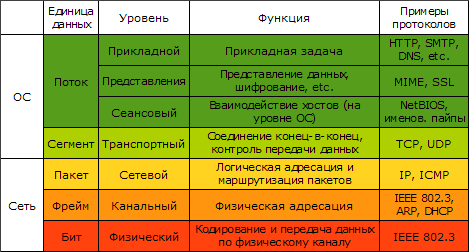
\includegraphics[width=0.8\textwidth]{img/exampleosi.png}
\caption{Описание модели OSI}
\label{fig1}
\end{figure}

Стек TCP/IP состоит из 4 слоев рис. \ref{fig2}:
\begin{enumerate}
\item Сетевой;
\item Интернета;
\item Транспортный;
\item Приложения;
\end{enumerate}

\begin{figure}[h!]
\centering
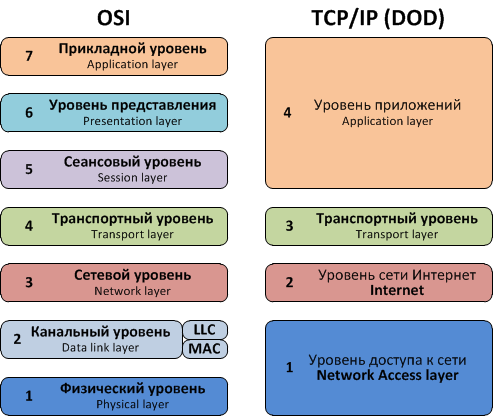
\includegraphics[width=0.8\textwidth]{img/ositcp.png}
\caption{Модель OSI и стек TCP/IP}
\label{fig2}
\end{figure}

\section{Отличия unicast anycast}

\begin{figure}[h!]
\centering
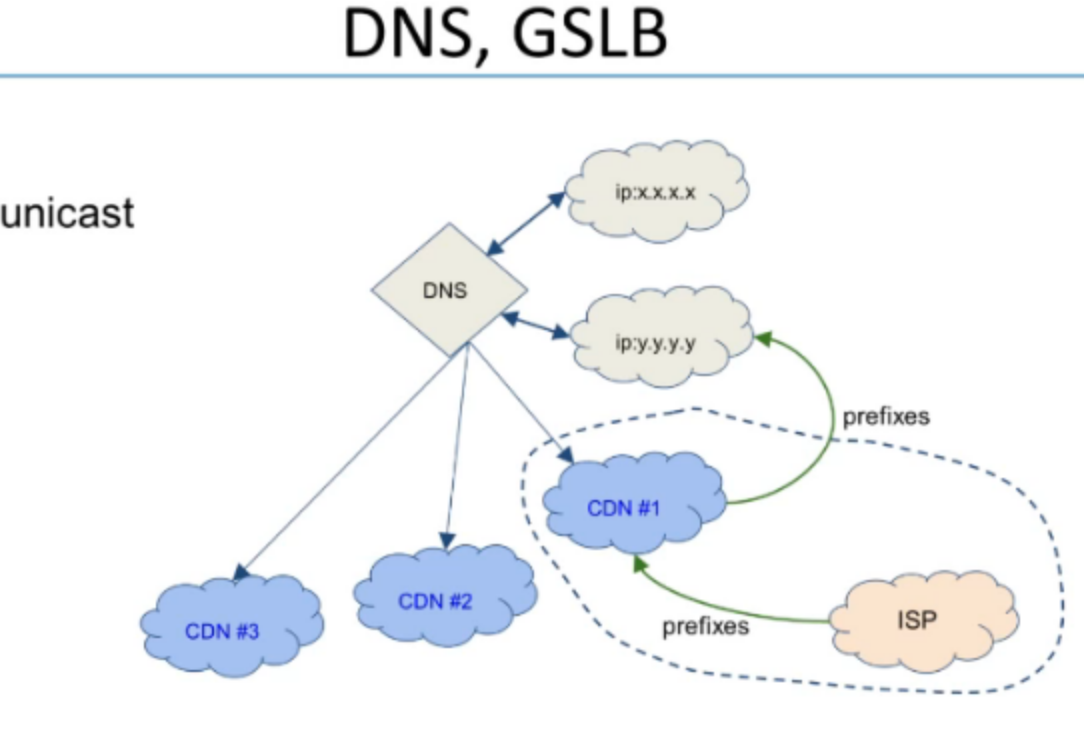
\includegraphics[width=0.8\textwidth]{img/unicast.png}
\caption{unicast}
\label{unicast}
\end{figure}

\section{Что такое CDN}

\section{Защита от SYN DDOS, Slow get/post, gzip bomb}

\section{Как избежать полного рукопажатия при tls?}

\section{Что такое BGP?}

\section{http 2?}

\section{websockets}

\begin{figure}[h!]
\centering
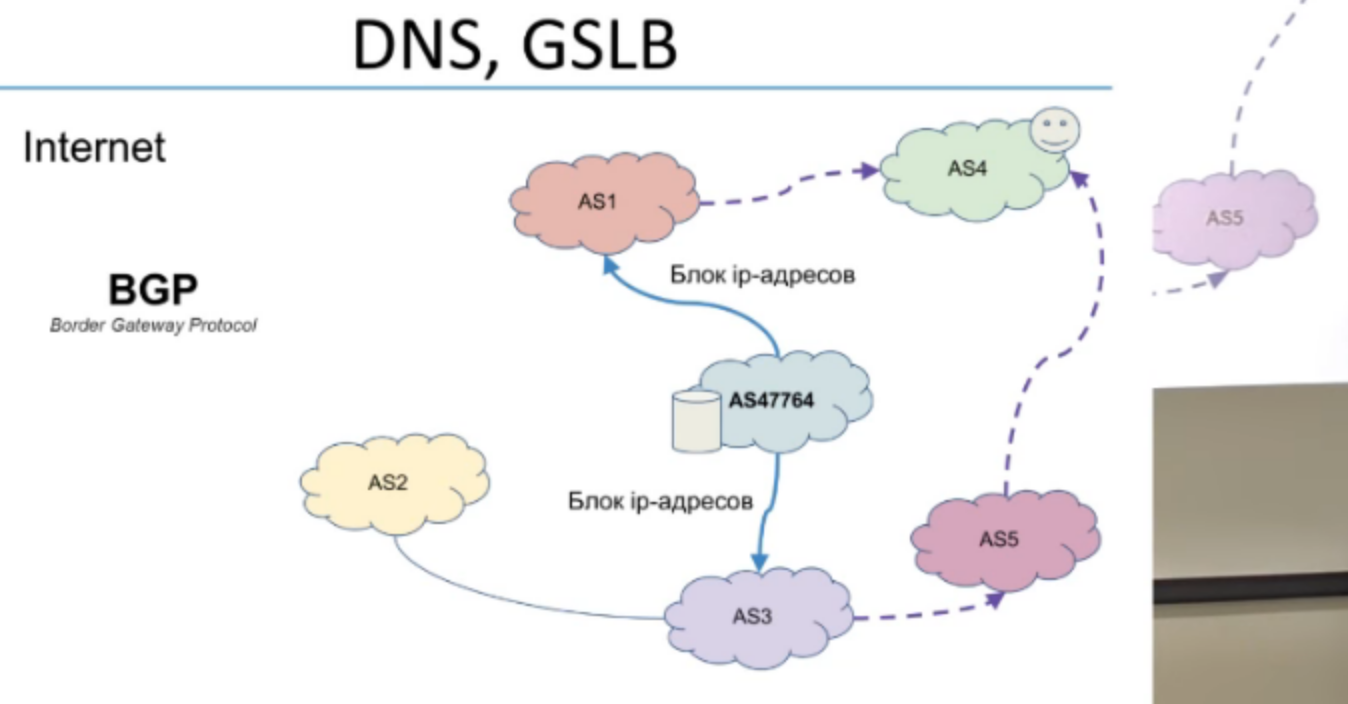
\includegraphics[width=0.8\textwidth]{img/BGP.png}
\caption{BGP}
\label{BGP}
\end{figure}

\chapter{Общие вопросы}

\section{Что такое DevOps}

DevOps (акроним от англ. development и operations) — это методология разработки ПО, сфокусированная на предельно активном взаимодействии и интеграции в одной упряжке программистов, тестировщиков и админов, синхронизировано обслуживающих общий для них сервис/продукт. Главная цель этого — создание единого цикла взаимозависимости разработки, эксплуатации и деплоя программного обеспечения, дабы в конечном счете помогать организациям (сервисам, стартапам) быстрее и безболезненней создавать и обновлять их программные продукты и сервисы, эксплуатируемые в режиме реального времени или «в продакшене».	

\section{Что такое Agile}
Agile — это не методология, а собирательное название различных методик и подходов к управлению, которые:

\begin{enumerate}
\item Фокусируют команду на нуждах и целях клиентов.
\item Упрощают оргструктуру и процессы.
\item Предлагают работу короткими циклами.
\item Активно используют обратную связь.
\item Предполагают повышение полномочий сотрудников.
\item Имеют в своей основе гуманистический подход.
\item Не являются конечным состоянием, а, скорее, образом мышления и жизни.
\end{enumerate}

\section{Что такое Kanban}

Канбан — это способ управления работой в духе Аджайла. Он содержит всего шесть правил и предлагает эволюционный переход от привычного образа мышления к аджайловому. Аджайл-коучи часто сравнивают Канбан с водой — он обтекает структуру и иерархию компании и медленно начинает их менять. Как вода точит камни, так Канбан меняет образ мышления.

\begin{enumerate}
\item Визуализируйте
\item Ограничивайте
\item Контролируйте
\item Договоритесь
\item Анализируйте
\item Экспериментируйте
\end{enumerate}


 \section{Типы балансировки, L3, L4, L7}
Распределение нагрузки по нескольким инстансам приложения.

\begin{figure}[h!]
\centering
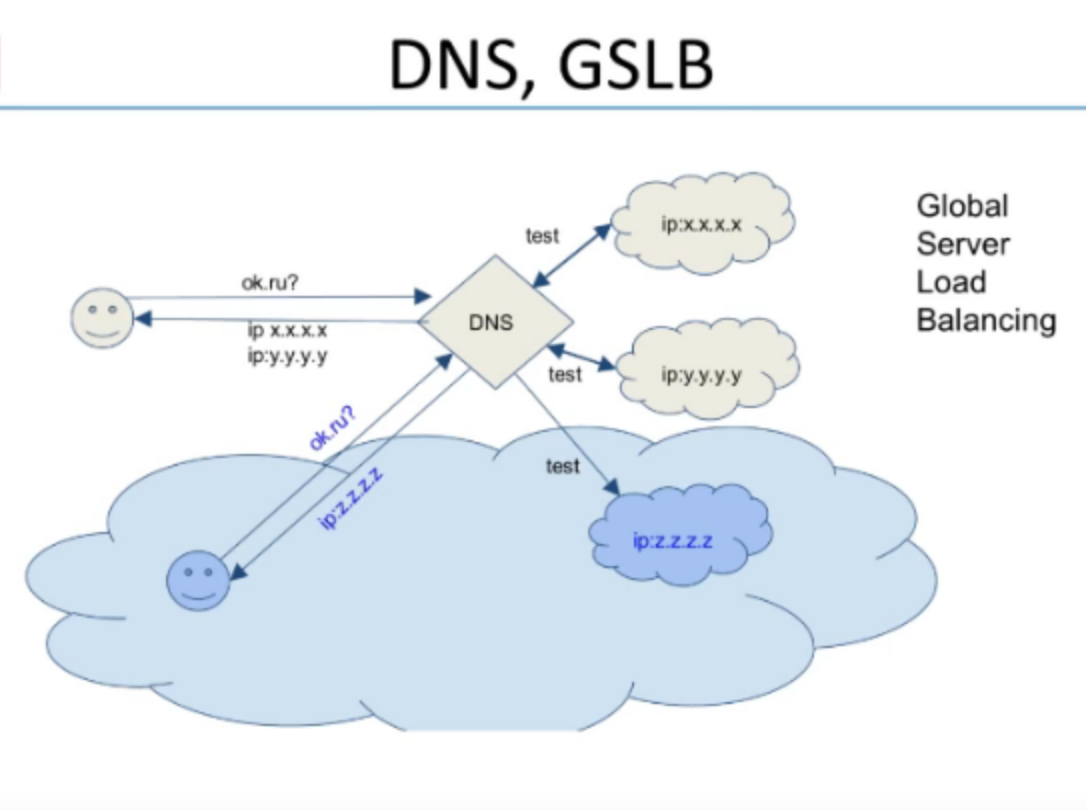
\includegraphics[width=0.8\textwidth]{img/balansing.png}
\caption{BGP}
\label{balansing}
\end{figure}
 
 \subsection{DNS Round Robin}
 Самый простой метод балансировки — это использование алгоритма DNS Round Robin. Суть его в том, что мы создаем несколько DNS-записей типа А для записи нашего домена на DNS-сервере. DNS-сервер выдает наши записи типа А в чередующемся циклическом порядке.
 
\subsection{Балансировка на втором уровне стека протоколов}     
 Следующий метод балансировки — это балансировка на втором уровне стека протоколов. Здесь можно выделить два варианта: балансировка с использованием отдельного выделенного балансировщика и без.

В обоих случаях мы берем некоторый IP-адрес нашего сервиса. Его мы устанавливаем для всех наших серверов либо на OBEC, либо на другой специализированный интерфейс. Делается это для того, чтобы данные серверы могли принимать соединения на этот IP-адрес и отвечать с него, но не отвечали бы на ARP-запросы, относящиеся к этому адресу.

Как работает такая балансировка? На балансировщик, имеющий этот IP-адрес и отвечающий на ARP, приходит, допустим, первый пакет соединения. Мы определяем, что он первый. Нужным алгоритмом отправляем его на интересующий нас сервер, меняя MAC-адрес на место назначения (англ. destination). Записываем его в некоторую таблицу соединений.

\subsection{Метод балансировки на третьем уровне}
Метод балансировки на третьем уровне стека протоколов, то есть на уровне протокола IP. В нем мы назначаем балансировщику тот же IP-адрес сервиса. Когда идет обращение на него, мы применяем так называемый Destination NAT, то есть подменяем IP-адрес назначения в пакете: IP-адреса текущего сервера меняется на выбранный по нужному алгоритму IP-адрес сервера, который будет обрабатывать запрос.

Отличие этого метода от предыдущего заключается в том, что мы модифицируем заголовки третьего уровня. Поэтому для ответов нам их также нужно модифицировать, провести обратную операцию замены. IP-адрес отправителя нужно поменять с IP-адреса сервера, который обрабатывает запрос, на IP-адрес сервиса, который используется на балансировщике.

\subsection{Метод проксирования}

Есть некоторый прокси-сервер, на котором используется IP-адрес нашего сервиса, он получает запрос, при необходимости что-то делает с ним и перенаправляет его уже от себя нужному серверу.

Этот метод для сервера уже не прозрачен, поскольку он видит, что к нему обращается наш прокси. Для этого внутри протокола высокого уровня мы должны каким-то образом передать сведения о том, какой же клиент к нам обращается. Для протокола HTTP мы можем добавлять заголовок X-Real-IP с IP-адресом клиента.

\subsection{Балансировка с помощью редиректа}
Есть некоторый балансировщик, который при обращении к нашему сервису (например, http://site.com) дает клиенту редирект на конкретный сервер (например, http://server2.site.com). В случае HTTP это будет выглядеть как "HTTP redirect 302", по-моему, код редиректа будет выглядеть как "временно перемещено" (англ. moved temporary).

\subsection{Балансировка L4}

\begin{figure}[h!]
\centering
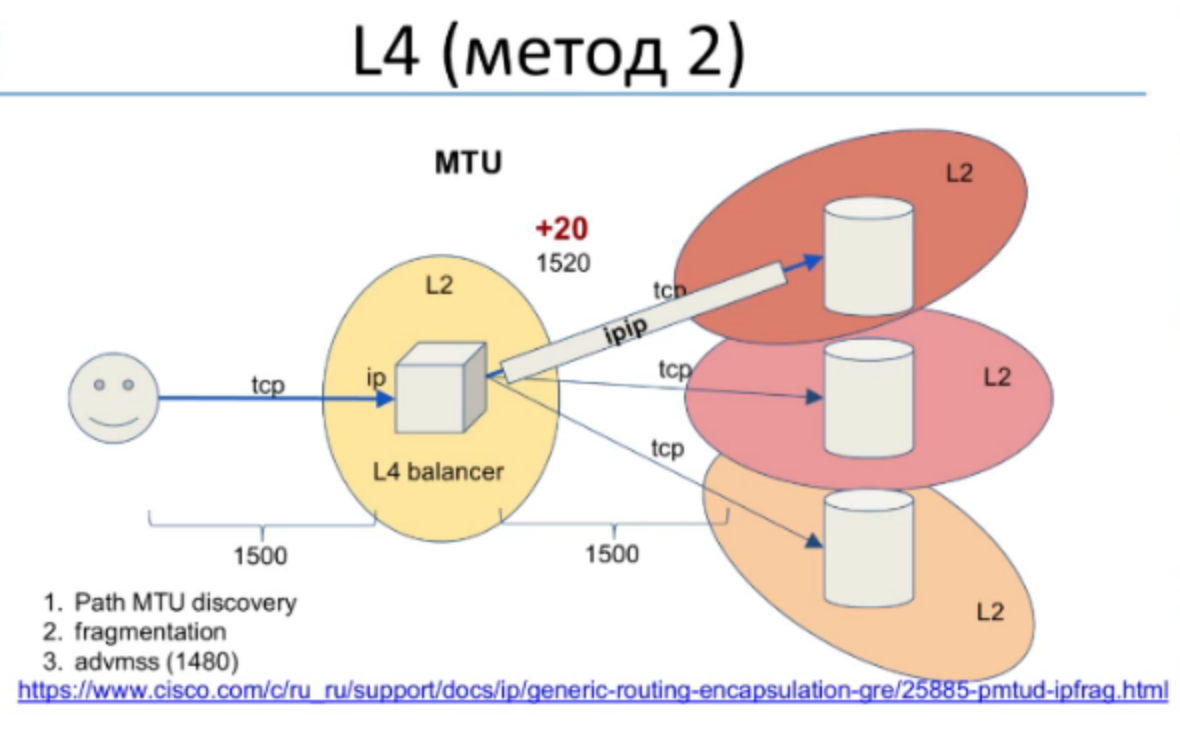
\includegraphics[width=0.8\textwidth]{img/L41.png}
\caption{Балансировка L4}
\label{L41}
\end{figure}


\begin{figure}[h!]
\centering
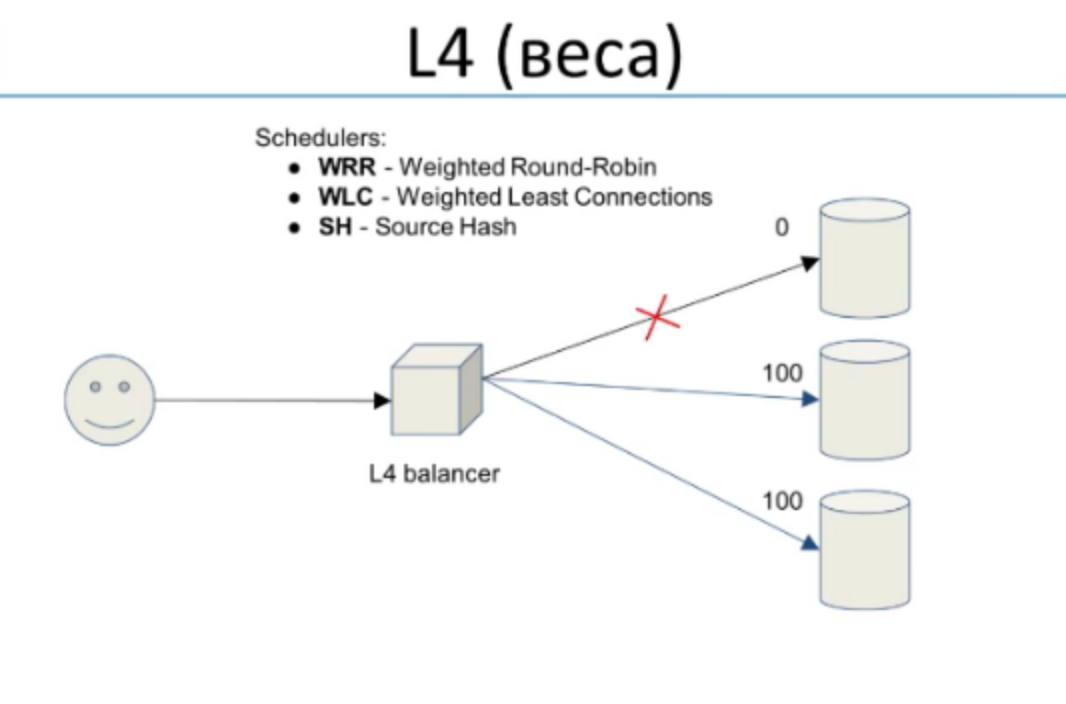
\includegraphics[width=0.8\textwidth]{img/L4-weights1.png}
\caption{Балансировка L4 c весами}
\label{L4w1}
\end{figure}


\begin{figure}[h!]
\centering
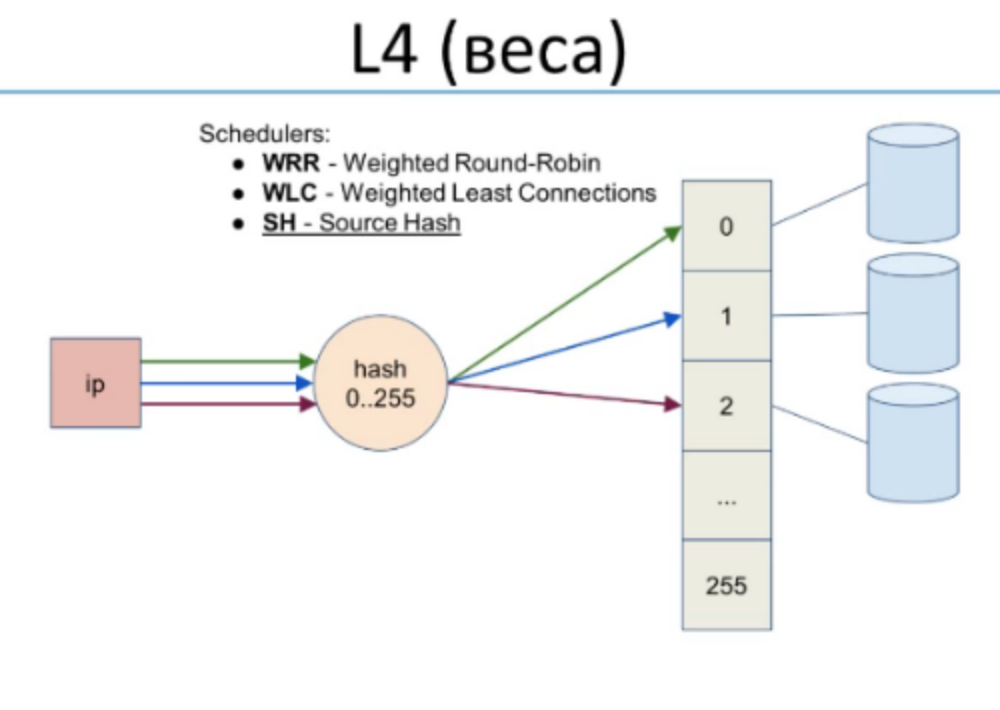
\includegraphics[width=0.8\textwidth]{img/L4-weights2.png}
\caption{Балансировка L4 с весами}
\label{L4w2}
\end{figure}

\section{Сине-зеленый деплой (blue-green deploy)}

Одна из задач автоматизации деплоя — переход из одного состояния в другое внутри себя же, с переводом софта из финальной стадии тестирования в действующий продакшен. Обычно это нужно сделать быстро, чтобы минимизировать время простоя. При \textbf{сине-зеленом подходе} у вас есть два продакшена, насколько возможно идентичных. В любое время один из них, допустим синий, активен. При подготовке новой версии софта, вы делаете финальное тестирование в зелёном продакшене. Вы убеждаетесь, что программа в этом продакшене работает и настраиваете роутер так, чтобы все входящие запросы шли в зелёную операционную среду — синяя в режиме ожидания.

\section{Какая разница между Continuous Delivery, Continuous Deployment и Continuous Integration}

\subsection{Continuous delivery (непрерывная доставка)}

В большинстве случаев непрерывная доставка — это серия практик, направленных на то, чтобы обновления программного обеспечения происходили практически постоянно. Данные методы гарантируют быстрое развёртывание на продакшене не меняя существующий функционал. Непрерывная доставка осуществима благодаря различным оптимизациям на ранних этапах процесса разработки.

Разработчик, сделав какую-либо фичу, отправляет её QA-инженерам для тестирования. Тестировщикам легче досконально оттестировать небольшой новый функционал и написать к нему тест-кейсы. Как только все проверки – прошли, новая фича попадает на дальнейшее тестирование авто-тестами и потом уже в релизный брэнч в системе контроля версий.


\subsection{Continuous deployment(непрерывное развёртываение)}

Continuous deployment часто путают с continuous delivery, хотя между ними существуют чёткие различия, которые следует знать и понимать.

Как выше было уже сказано непрерывная доставка обеспечивает постоянный выпуск обновлений пользователям. А непрерывное развёртывание отвечает за то, чтобы весь новый функционал после тестирования сразу же попал в основную программу без ручного вмешательства инженеров DevOps.

Тот же Docker создан для неприрывного развёртывания. DevOps инженеры могут обновлять контейнеры и разворачивать их сразу на продакшене в автоматическом режиме. Такой процесс является ключом к непрерывной доставке, т.к. весь процесс может занять всего лишь несколько минут.

Не всегда непрерывное развёртывание имеет смысл. Использование фича-тоглинга сводит на нет все преимущества. Всегда надо исходить из потребностей бизнеса и процессов внедрения нового функционала.

\subsection{Continuous integration (непрерывная интеграция)}

Непрерывная интеграция является ключевым компонентом практики Agile Development. Основой данной практики является постоянное попадание кода в центральный репозиторий после успешного запуска тестов. Основные цели continuous integration – поиск и устранение потенциальных проблем как можно быстрее, улучшение качества ПО и сокращение время для выпуска обновлений.

До того, как непрерывная интеграция стала широко распространённой, разработчики обычно работали изолировано, а только по окончанию работы объедениняли свои наработки. Порой это был очень трудоёмкий и длительный процесс.

При непрерывной интеграции разработчики часто заливают свои изменения в центральный репозиторий, выполняя до этого unit – тесты. Затем система контроля версий автоматически проверяет код на возможно безопасной интеграции с существующим в репозитории. При этом идёт постоянное поступление кода, что облегчает тестирование и сводит к минимуму возможные риски.

\begin{figure}[h!]
\centering
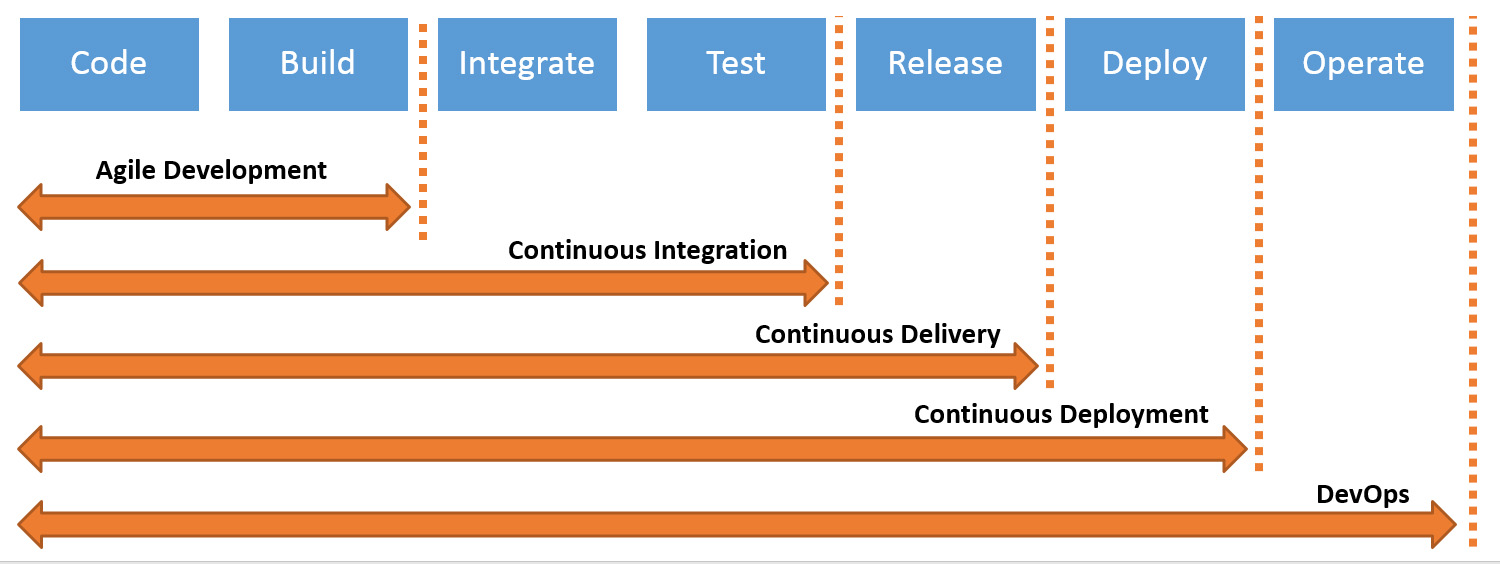
\includegraphics[width=0.9\textwidth]{img/ci-vs-cd-devops-difference.jpg}
\caption{Сравнение CI CD}
\label{fig5}
\end{figure}

\section{Как в access логе посмотреть самые активные ip за сутки}

\begin{lstlisting}
awk '{print $1, $9}' gitlab_access.log | uniq -c | sort -nk1 -r
\end{lstlisting}

\section{Системы управления конфигурациями Ansible/Puppet/Chef}
\section{CI системы Jenkins/TeamCity}
\section{Cтеком Hashicorp (Vault, Consul, Nomad, Teпaform}
\textbf{Vault} - хранилище секретов.

\textbf{Consul} предназначен для service discovery, как и, например, etcd или ZooKeeper. Но далеко не всем известно, что помимо service discovery также Consul имеет огромное количество других возможностей, например, встроенный мониторинг сервисов, распределенные локи, и другие. 
\section{Стек ELK (elasticsearch, logstash, kibana)}
\subsection{logstash}
logstash – это утилита для сборки, фильтрации и последующего перенаправления в конечное хранилище данных. Вы могли слышать о fluentd – logstash решает ту же самую задачу, но написан на jruby и чуть более лучше дружит с elasticsearch.
\subsection{elasticsearch}
Изначально, elasticsearch – это решение для полнотекстового поиска, построенное поверх Apache Lucene, но с дополнительными удобствами, типа лёгкого масштабирования, репликации и прочих радостей, которые сделали elasticsearch очень удобным и хорошим решением для высоконагруженных проектов с большими объёмами данных.
\subsection{kibana}
И вот у нас есть logstash, который собирает и обрабатывает данные со всех ваших тысяч серверов и elasticsearch, который изо всех сил эти данные хранит и позволяет искать по ним. Чего не хватает? Верно, не хватает Angular.js.

Поэтому в какой-то момент товарищ Rashid Khan написал для elasticsearch красивое Angular.js приложение kibana, позволяющее брать/искать данные по elasticsearch и строить множество красивых графиков. Ребята из elasticsearch не дураки, поэтому, увидев всё удобство этого решения, они забрали разработчика kibana к себе на борт.
\section{AWS, GCP, Azure, OpenStack}
\section{Vargant}
\section{Ситема мониторинга Prometheus (pull)/Collectd (push)/Grafana}

\section{Вывести ip и/или email nginx}

\begin{lstlisting}
less /var/log/nginx/access.log | cut -d' ' -f1 | sort | uniq -c
grep -E -o "\b[A-Za-z0-9._%+-]+@[A-Za-z0-9.-]+\.[A-Za-z]{2,6}\b" file.txt
awk '{print $1, $9}' gitlab_access.log | sort -u -nk1 
\end{lstlisting}

\section{Постраничный вывод файла}
\begin{lstlisting}
while read LINE; do echo "$LINE" | cut -f1 -d":"; done < /etc/passwd
\end{lstlisting}

\chapter{Разное}

\section{Различия точек обмена RabbitMQ}

Есть несколько типов точек доступа:

\begin{itemize}
\item \textbf{прямые (direct)}

Точки доступа типа direct работают по принципу привязки по ключу. У сообщения есть routing key, а у очереди есть binding key. Сообщения доставляются только в ту очередь, с которой точь-в-точь совпадают ключи.
\item \textbf{множественные (fanout)}

Точки доступа типа fanout отправляют сообщения во все очереди, которые созданы в этой точке. К слову сказать, если в direct exchange создать несколько разных очередей с одинаковым ключом, то они будут работать по принципу fanout: сообщения, у которых routing key будет совпадать, будут приходить во все очереди с таким же binding key.
\item \textbf{обратные (topic)}

Точки доступа типа topic проверяют специальные символы между ключом сообщения и шаблоном (routing pattern), который участвует в привязке очереди.
\item \textbf{заголовочные (header)}

Точки доступа типа header для маршрутизации используют атрибуты в заголовках сообщений.
\end{itemize}

\begin{figure}[h!]
\centering
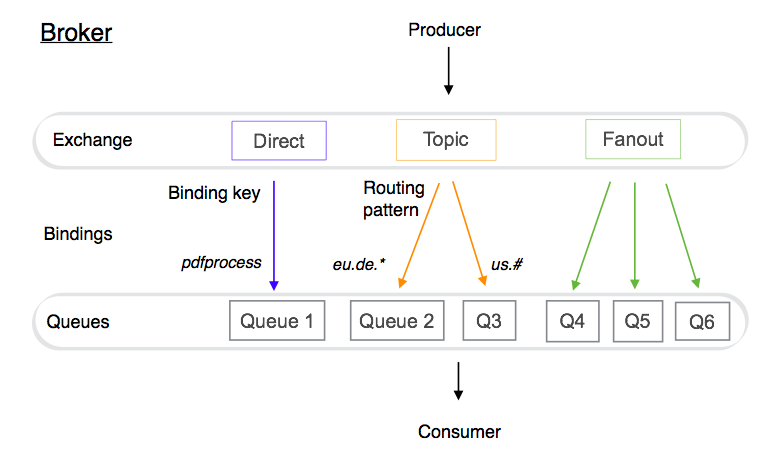
\includegraphics[width=0.9\textwidth]{img/exchanges.png}
\caption{Различия exchanges}
\label{fig6}
\end{figure}

\section{Отличия RabbitMQ и Kafka по гарантии доставке сообщений?}
\section{Области памяти стек и куча}

\begin{figure}[h!]
\centering
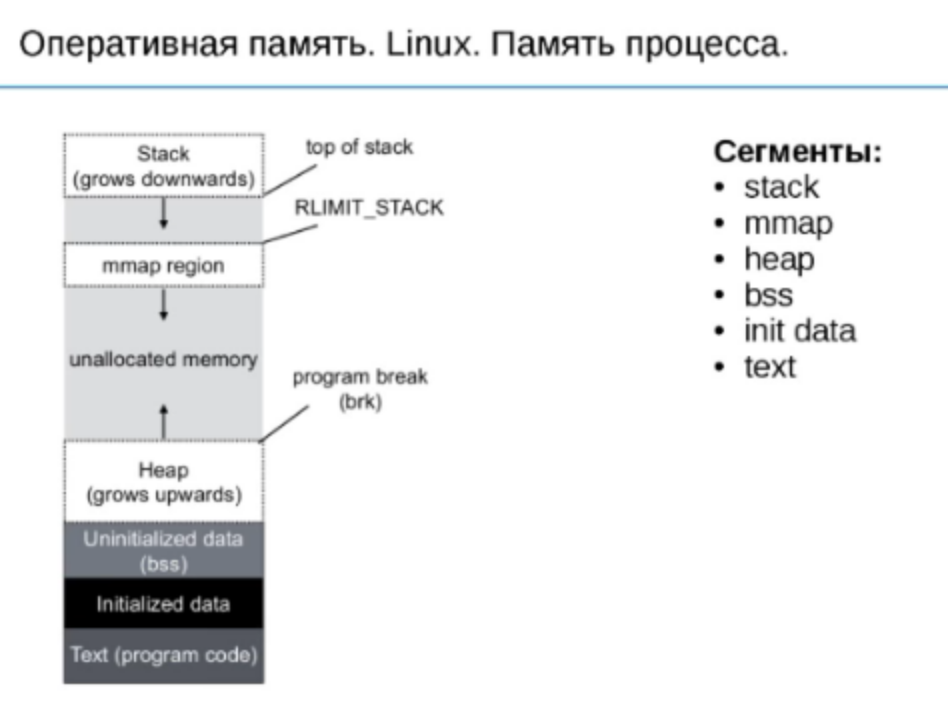
\includegraphics[width=0.8\textwidth]{img/memory.png}
\caption{Memory}
\label{memory}
\end{figure}

\subsection{Стек}

Стек — это область оперативной памяти, которая создаётся для каждого потока. Он работает в порядке LIFO (Last In, First Out),  то есть последний добавленный в стек кусок памяти будет первым в очереди на вывод из стека. Каждый раз, когда функция объявляет новую переменную, она добавляется в стек, а когда эта переменная пропадает из области видимости (например, когда функция заканчивается), она автоматически удаляется из стека. Когда стековая переменная освобождается, эта область памяти становится доступной для других стековых переменных.

Из-за такой природы стека управление памятью оказывается весьма логичным и простым для выполнения на ЦП; это приводит к высокой скорости, в особенности потому, что время цикла обновления байта стека очень мало, т.е. этот байт скорее всего привязан к кэшу процессора. Тем не менее, у такой строгой формы управления есть и недостатки. Размер стека — это фиксированная величина, и превышение лимита выделенной на стеке памяти приведёт к переполнению стека. Размер задаётся при создании потока, и у каждой переменной есть максимальный размер, зависящий от типа данных. Это позволяет ограничивать размер некоторых переменных (например, целочисленных), и вынуждает заранее объявлять размер более сложных типов данных (например, массивов), поскольку стек не позволит им изменить его. Кроме того, переменные, расположенные на стеке, всегда являются локальными.

В итоге стек позволяет управлять памятью наиболее эффективным образом — но если вам нужно использовать динамические структуры данных или глобальные переменные, то стоит обратить внимание на кучу.

\subsection{Куча}

Куча — это хранилище памяти, также расположенное в ОЗУ, которое допускает динамическое выделение памяти и не работает по принципу стека: это просто склад для ваших переменных. Когда вы выделяете в куче участок памяти для хранения переменной, к ней можно обратиться не только в потоке, но и во всем приложении. Именно так определяются глобальные переменные. По завершении приложения все выделенные участки памяти освобождаются. Размер кучи задаётся при запуске приложения, но, в отличие от стека, он ограничен лишь физически, и это позволяет создавать динамические переменные.

Вы взаимодействуете с кучей посредством ссылок, обычно называемых указателями — это переменные, чьи значения являются адресами других переменных. Создавая указатель, вы указываете на местоположение памяти в куче, что задаёт начальное значение переменной и говорит программе, где получить доступ к этому значению. Из-за динамической природы кучи ЦП не принимает участия в контроле над ней; в языках без сборщика мусора (C, C++) разработчику нужно вручную освобождать участки памяти, которые больше не нужны. Если этого не делать, могут возникнуть утечки и фрагментация памяти, что существенно замедлит работу кучи.

В сравнении со стеком, куча работает медленнее, поскольку переменные разбросаны по памяти, а не сидят на верхушке стека. Некорректное управление памятью в куче приводит к замедлению её работы; тем не менее, это не уменьшает её важности — если вам нужно работать с динамическими или глобальными переменными, пользуйтесь кучей.

\section{Прогрев кешей}

\section{Из каких базовых вещей состоят контейнеры: namespaces, cgroups}
	Все инструменты контейнеризации — будь то Docker, LXC или systemd-nspawn,— основываются на двух подсистемах ядра Linux: namespaces и cgroups. 
	
	\subsection{chroot}
	
	Идеи, лежащие в основе механизма пространств имён, не новы. Ещё в 1979 году в UNIX был добавлен системный вызов chroot() — как раз с целью обеспечить изоляцию и предоставить разработчикам отдельную от основной системы площадку для тестирования. 
	
	Название chroot представляет собой сокращение от change root, что дословно переводится как «изменить корень». С помощью системного вызова chroot() и соответствующей команды можно изменить корневой каталог. Программе, запущенной с изменённым корневым каталогом, будут доступны только файлы, находящиеся в этом каталоге. 
	
	Вершиной этой иерархии является каталог /, он же root. Все остальные каталоги — usr, local, bin и другие, — связаны с ним.

С помощью chroot в систему можно добавить второй корневой каталог, который с точки зрения пользователя ничем не будет отличаться от первого. Файловую систему, в которой присутствует изменённый корневой каталог, можно схематично представить на рис. \ref{3}.

\begin{figure}[h!]
\centering
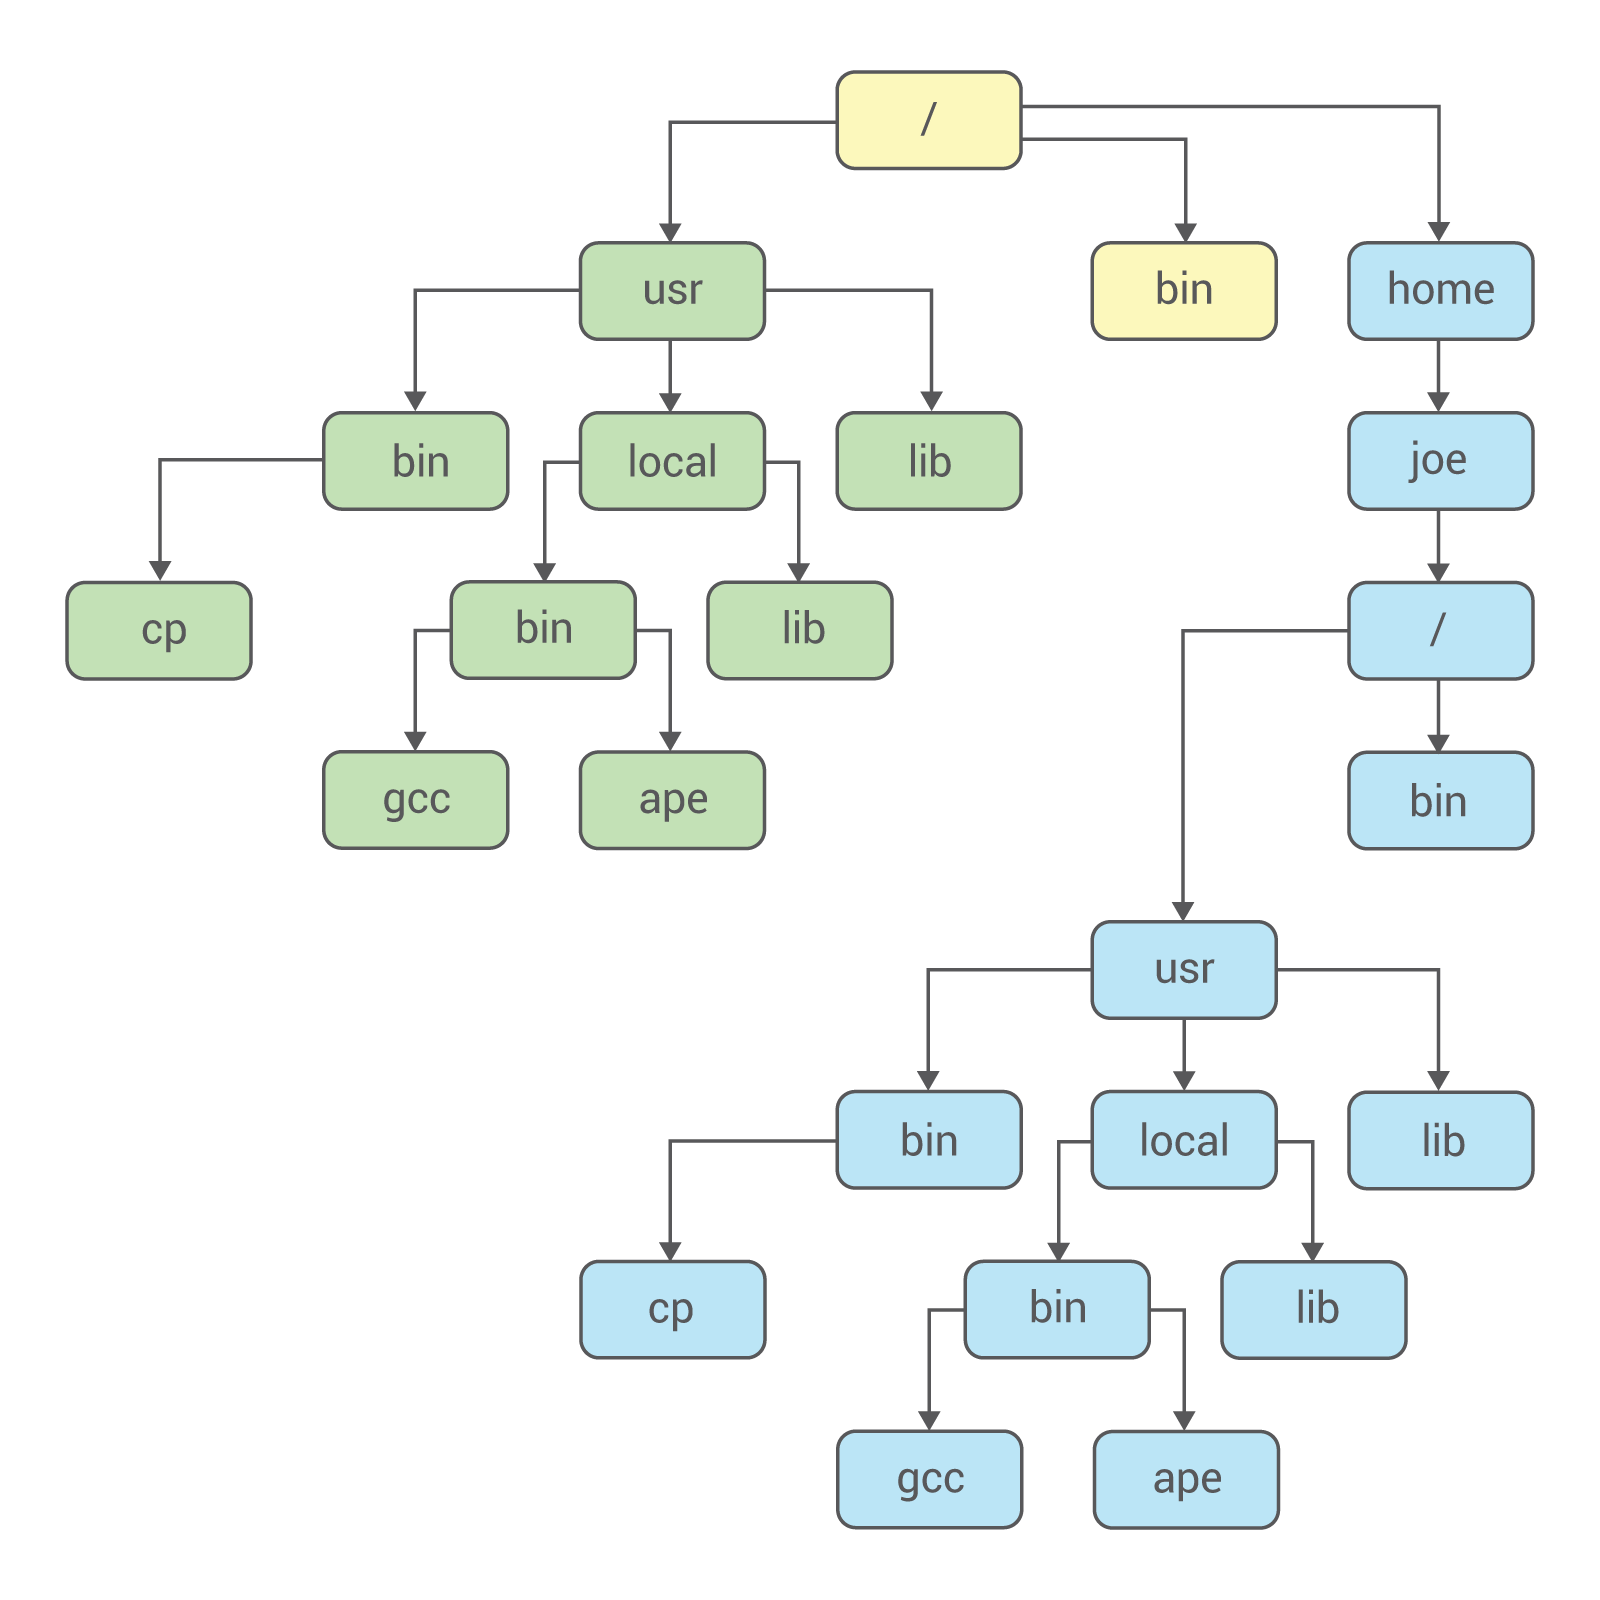
\includegraphics[width=0.9\textwidth]{img/chroot.png}
\caption{Представление файловой системы linux}
\label{fig3}
\end{figure}

\subsection{namespaces}

Пространство имён (англ. namespace) — это механизм ядра Linux, обеспечивающий изоляцию процессов друг от друга. Работа по его реализации была начата в версии ядра 2.4.19. На текущий момент в Linux поддерживается шесть типов пространств имён:

\begin{table}[]
\begin{tabular}{|l|l|}
\hline
Пространство имен & Что изолирует  \\ \hline
PID & PID процессов  \\ \hline
NETWORK & Сетевые устройства, стеки, порты... \\ \hline
USER & ID пользователей и групп \\ \hline
MOUNT & Точки монтирования \\ \hline
IPC & SystemV IPC, очереди сообщений POSIX \\ \hline
UTS & Имя хоста и доменное имя NIS \\ \hline
\end{tabular}
\end{table}

Неймспейсы изолируют друг от другая процессы таким образом, что процессы в одной группе не могут видеть ресурсы другой группы. Например, PID namespace предоставляет уникальные идентификаторы процессов в рамках группы. Внутри одной группы может быть процесс с pid 1 и внутри второй группы тоже может быть процесс с pid 1, хотя это два совершенно разных процесса, которые друг о другие ничего не знают. Притом, все процессы все также имеют уникальные id в рамках ОС. Просто, если смотреть на процессы из группы, то эти id отображаются в другие.

\subsubsection{PID: изоляция PID процессов}

При загрузке в Linux сначала запускается процесс с идентификационным номером (PID) 1. В дереве процессов он является корневым. Он запускает другие процессы и службы. Механизм namespaces позволяет создавать отдельное ответвление дерева процессов с собственным PID 1. Процесс, который создаёт такое ответвление, являются частью основного дерева, но его дочерний процесс уже будет корневым в новом дереве.

Процессы в новом дереве никак не взаимодействуют с родительским процессом и даже не «видят» его. В то же время процессам в основном дереве доступны все процессы дочернего дерева. Наглядно это показано на рис.

\begin{figure}[h!]
\centering
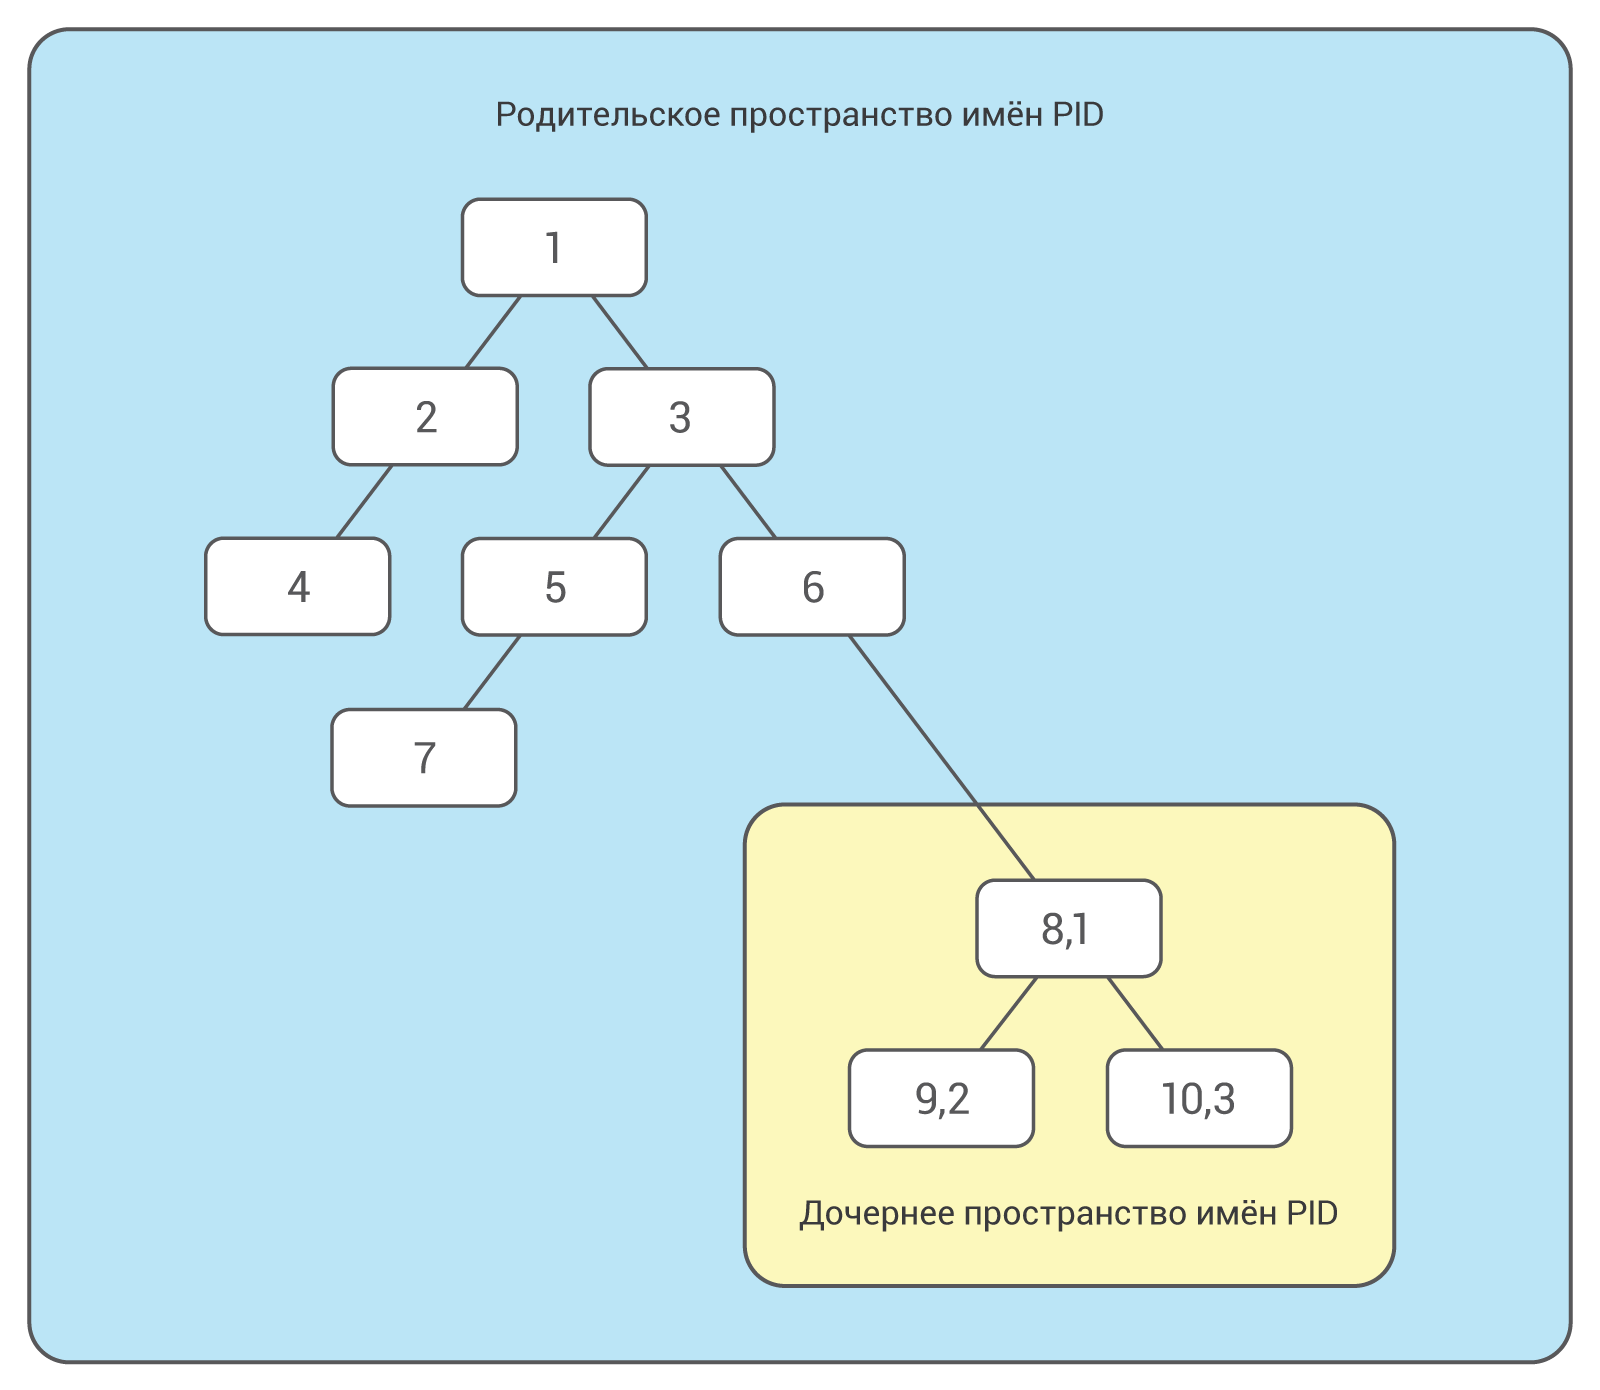
\includegraphics[width=0.9\textwidth]{img/pid.png}
\caption{Представление файловой системы linux}
\label{fig4}
\end{figure}

\subsubsection{NET: изоляция сетей}

Благодаря пространству имён NET мы можем выделять для изолированных процессов собственные сeтевые интерфейсы. Даже loopback-интерфейс для каждого пространства имён будет отдельным.

Сетевые пространства имён можно создавать с помощью системного вызова clone() с флагом CLONE\_NEWNET. 

\subsubsection{MOUNT: изоляция файловой системы}

Об изоляции на уровне файловой системы мы уже упоминали выше, когда разбирали системный вызов chroot (). Мы отметили, что системный вызов chroot() не обеспечивает надёжной изоляции. С помощью же пространств имён MOUNT можно создавать полностью независимые файловые системы, ассоциируемые с различными процессами.

\subsection{cgroups (Control Groups)}

Позволяют организовывать процессы в группы и для каждой группы задавать лимиты. Например, лимиты на использование CPU, объем используемой памяти и дисковый ввод-вывод.

Механизм cgroups состоит из двух составных частей: ядра (cgroup core) и так называемых подсистем. В ядре версии 4.4.0.21 таких подсистем 12:

\begin{itemize}
   \item blkio — устанавливает лимиты на чтение и запись с блочных устройств;
    \item cpuacct — генерирует отчёты об использовании ресурсов процессора;
    \item cpu — обеспечивает доступ процессов в рамках контрольной группы к CPU;
    \item cpuset — распределяет задачи в рамках контрольной группы между процессорными ядрами;
    \item devices — разрешает или блокирует доступ к устройствам;
    \item freezer — приостанавливает и возобновляет выполнение задач в рамках контрольной группы
    \item hugetlb — активирует поддержку больших страниц памяти для контрольных групп;
    \item memory — управляет выделением памяти для групп процессов;
    \item net\_cls — помечает сетевые пакеты специальным тэгом, что позволяет идентифицировать пакеты, порождаемые определённой задачей в рамках контрольной группы;
    \item netprio — используется для динамической установки приоритетов по трафику;
    \item pids — используется для ограничения количества процессов в рамках контрольной группы.
\end{itemize}

Каждая подсистема представляет собой директорию с управляющими файлами, в которых прописываются все настройки.  

\subsection{Отличия namespaces от cgroups}

\textbf{cgroup}: Контрольные группы предоставляют механизм для агрегирования или разбиения наборов задач и всех их будущих детей в иерархические группы со специализированным поведением.
\textbf{namespace}: обертывает глобальный системный ресурс в абстракции, которая заставляет его казаться процессам в пространстве имен, что у них есть свой отдельный экземпляр глобального ресурса.

\textbf{Вкратце}:

     cgroups = ограничивает, сколько вы можете использовать;
     namespaces = пределы того, что вы можете видеть (и, следовательно, использовать)

\section{Времена доступа}

\begin{figure}[h!]
\centering
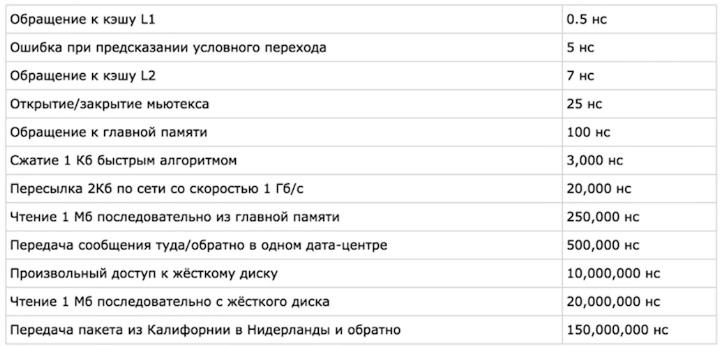
\includegraphics[width=0.8\textwidth]{img/time.png}
\caption{Time}
\label{time}
\end{figure}
